\part{Neural networks}
\frame{\partpage}

\begin{frame}{Artificial Neural Networks (ANNs)}
	\begin{itemize}
		\pause\item \textbf{Inspired by} the structure of biological brains
		\pause\item Idea has been around since the 1950s
		\pause\item Recent resurgence of interest: today's powerful CPUs and GPUs allow much larger ANNs to be used
	\end{itemize}
\end{frame}

\begin{frame}{Real neurons}
	\begin{columns}
		\begin{column}{0.48\textwidth}
			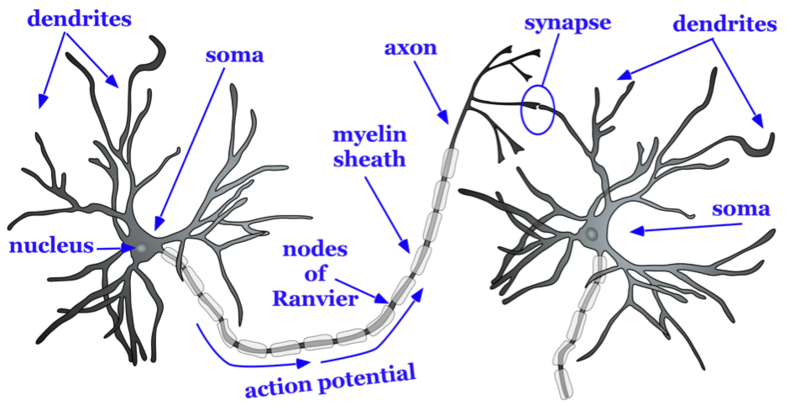
\includegraphics[width=\textwidth]{neuron}
		\end{column}
		\begin{column}{0.48\textwidth}
			\begin{itemize}
				\pause\item An \textbf{electrically excitable} cell
				\pause\item Neurons are \textbf{connected together}
				\pause\item Connections can be \textbf{excitatory} or \textbf{inhibitory}
			\end{itemize}
		\end{column}
	\end{columns}
	\begin{itemize}
		\pause\item If enough excitatory signals are received, the neuron \textbf{fires} ---
			sends an electrical signal to the connected neurons
		\pause\item Human brain contains approximately \textbf{100 billion} neurons
	\end{itemize}
\end{frame}

\begin{frame}{An artificial neuron}
	\begin{columns}
		\begin{column}{0.48\textwidth}
			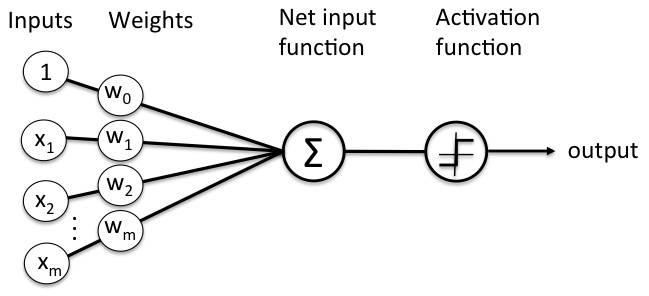
\includegraphics[width=\textwidth]{perceptron}
		\end{column}
		\begin{column}{0.48\textwidth}
			\begin{itemize}
				\pause\item A \textbf{perceptron}
				\pause\item Inputs $x_1, \dots, x_m$ are outputs from \textbf{other perceptrons}
				\pause\item Each input has a \textbf{weight} $w_i$ between $-1$ and $+1$
			\end{itemize}
		\end{column}
	\end{columns}
\end{frame}

\begin{frame}{Perceptron activation}
	\begin{itemize}
		\pause\item The perceptron calculates a \textbf{weighted sum}
			$$ w_0 + w_1 x_1 + \dots + w_m x_m $$
		\pause\item This goes through an \textbf{activation function}
		\pause\item Simplest: \textbf{step function}
			$$ \textbf{output} = \begin{cases}
				1 &\text{ if sum $\geq$ threshold} \\
				0 &\text{ if sum $<$ threshold}
			\end{cases}
			$$
		\pause\item More common: \textbf{sigmoid function}
	\end{itemize}
	\begin{center}
		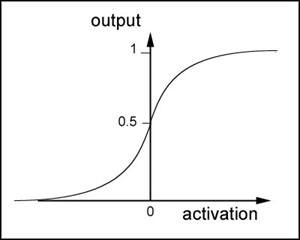
\includegraphics[width=0.3\textwidth]{sigmoid}
	\end{center}
\end{frame}

\begin{frame}{An artificial neural network}
	\begin{columns}
		\begin{column}{0.48\textwidth}
			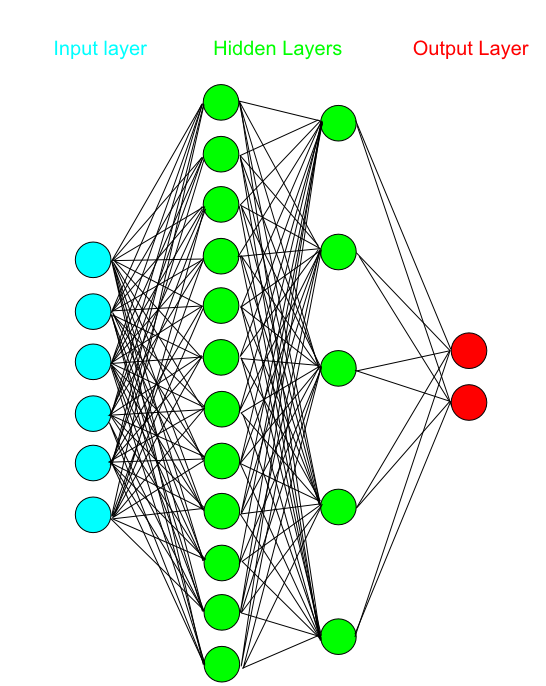
\includegraphics[width=\textwidth]{multilayer_perceptron}
		\end{column}
		\begin{column}{0.48\textwidth}
			\begin{itemize}
				\pause\item A \textbf{multilayer perceptron (MLP)}
				\pause\item Consists of an \textbf{input layer}, several \textbf{hidden layers} and an \textbf{output layer}
				\pause\item Each layer is an array of \textbf{perceptrons}
				\pause\item Each perceptron's output is connected to \textbf{every} perceptron in the next layer
			\end{itemize}
		\end{column}
	\end{columns}
\end{frame}

\begin{frame}{Image classification}
	\begin{columns}
		\begin{column}{0.48\textwidth}
			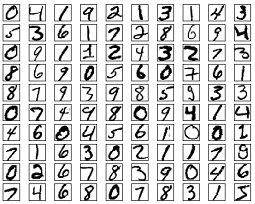
\includegraphics[width=\textwidth]{mnist_100_digits}
		\end{column}
		\begin{column}{0.48\textwidth}
			\begin{itemize}
				\pause\item Classic example: \textbf{handwritten digit recognition}
				\pause\item Given a \textbf{raster image}, which of the digits 0 to 9 does it represent?
			\end{itemize}
		\end{column}
	\end{columns}
\end{frame}

\begin{frame}
	\begin{center}
		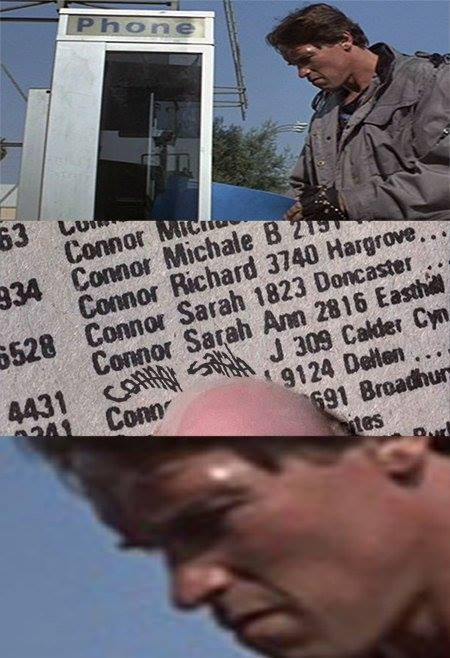
\includegraphics[height=0.8\textheight]{captcha}

		\tiny{\url{https://twitter.com/NaughtThought/status/846262063827730432}}
	\end{center}
\end{frame}

\begin{frame}{MLPs for image classification}
	\begin{itemize}
		\pause\item \textbf{Input}: pixels of the image, reduced down to 1 bit per pixel (i.e.\ black or white)
			\begin{itemize}
				\pause\item Input layer: 1 perceptron per pixel
			\end{itemize}
		\pause\item \textbf{Output}: 10 bits corresponding to digits 0 to 9, of which exactly one should be set
			\begin{itemize}
				\pause\item Output layer: 10 perceptrons
			\end{itemize}
		\pause\item \textbf{Hidden layers}: ???
			\begin{itemize}
				\pause\item Parameters to tune
			\end{itemize}
		\pause\item \textbf{Weights}: ???
	\end{itemize}
\end{frame}

\begin{frame}{How to set the weights?}
	\begin{itemize}
		\pause\item We need to \textbf{train} the network
		\pause\item Idea:
			\begin{itemize}
				\pause\item Feed in \textbf{training data}
				\pause\item When the network happens to give the correct answer, \textbf{reinforce}
					the relevant weights
				\pause\item Repeat until a desired \textbf{accuracy} is obtained
			\end{itemize}
		\pause\item Note: this requires a large amount of training data that is \textbf{tagged},
			i.e.\ for which we already know the correct answer
	\end{itemize}
\end{frame}

\begin{frame}{Stochastic gradient descent}
	\begin{itemize}
		\pause\item \textbf{Gradient descent}: opposite of \textbf{gradient ascent} a.k.a.\ \textbf{hillclimbing}
		\pause\item Want to minimise the \textbf{error} over the training data
		\pause\item \textbf{Stochastic}: perform several training \textbf{epochs}
		\pause\item Each epoch uses a randomly sampled \textbf{subset} of the training data
		\pause\item This reduces computation time, and helps to escape local optima
	\end{itemize}
\end{frame}

\begin{frame}{ANN example}
	\begin{center}
		\url{http://playground.tensorflow.org}
	\end{center}
\end{frame}

\begin{frame}{Overfitting}
	\begin{itemize}
		\pause\item ANN learns \textbf{patterns} in the training data
		\pause\item Insufficient training data might result in the network learning ``patterns''
			that are actually random anomalies
	\end{itemize}
\end{frame}
